\documentclass[10pt,twocolumn]{article}\usepackage[]{graphicx}\usepackage[]{color}
% maxwidth is the original width if it is less than linewidth
% otherwise use linewidth (to make sure the graphics do not exceed the margin)
\makeatletter
\def\maxwidth{ %
  \ifdim\Gin@nat@width>\linewidth
    \linewidth
  \else
    \Gin@nat@width
  \fi
}
\makeatother

\definecolor{fgcolor}{rgb}{0.345, 0.345, 0.345}
\newcommand{\hlnum}[1]{\textcolor[rgb]{0.686,0.059,0.569}{#1}}%
\newcommand{\hlstr}[1]{\textcolor[rgb]{0.192,0.494,0.8}{#1}}%
\newcommand{\hlcom}[1]{\textcolor[rgb]{0.678,0.584,0.686}{\textit{#1}}}%
\newcommand{\hlopt}[1]{\textcolor[rgb]{0,0,0}{#1}}%
\newcommand{\hlstd}[1]{\textcolor[rgb]{0.345,0.345,0.345}{#1}}%
\newcommand{\hlkwa}[1]{\textcolor[rgb]{0.161,0.373,0.58}{\textbf{#1}}}%
\newcommand{\hlkwb}[1]{\textcolor[rgb]{0.69,0.353,0.396}{#1}}%
\newcommand{\hlkwc}[1]{\textcolor[rgb]{0.333,0.667,0.333}{#1}}%
\newcommand{\hlkwd}[1]{\textcolor[rgb]{0.737,0.353,0.396}{\textbf{#1}}}%
\let\hlipl\hlkwb

\usepackage{framed}
\makeatletter
\newenvironment{kframe}{%
 \def\at@end@of@kframe{}%
 \ifinner\ifhmode%
  \def\at@end@of@kframe{\end{minipage}}%
  \begin{minipage}{\columnwidth}%
 \fi\fi%
 \def\FrameCommand##1{\hskip\@totalleftmargin \hskip-\fboxsep
 \colorbox{shadecolor}{##1}\hskip-\fboxsep
     % There is no \\@totalrightmargin, so:
     \hskip-\linewidth \hskip-\@totalleftmargin \hskip\columnwidth}%
 \MakeFramed {\advance\hsize-\width
   \@totalleftmargin\z@ \linewidth\hsize
   \@setminipage}}%
 {\par\unskip\endMakeFramed%
 \at@end@of@kframe}
\makeatother

\definecolor{shadecolor}{rgb}{.97, .97, .97}
\definecolor{messagecolor}{rgb}{0, 0, 0}
\definecolor{warningcolor}{rgb}{1, 0, 1}
\definecolor{errorcolor}{rgb}{1, 0, 0}
\newenvironment{knitrout}{}{} % an empty environment to be redefined in TeX

\usepackage{alltt}
\usepackage[british]{babel}
%\usepackage[utf8]{inputenc}
\usepackage[margin=2.25cm]{geometry}
\usepackage{graphicx}
\usepackage{listings}
\usepackage{subcaption}
\usepackage{float}
\usepackage{hyperref}
\usepackage[table,xcdraw]{xcolor}
\usepackage[ruled,vlined]{algorithm2e}
\usepackage{setspace}
\usepackage{verbatim}
\usepackage{booktabs}
\usepackage{titlesec}

%argmin, argmax
\usepackage{amsmath}
\DeclareMathOperator*{\argmax}{arg\,max}
\DeclareMathOperator*{\argmin}{arg\,min}
\DeclareMathOperator*{\diag}{diag}

\newcommand{\mmatrix}[1]{\boldsymbol{#1}}
\newcommand{\mvec}[1]{\boldsymbol{#1}}

\graphicspath{ {./images/} }

\usepackage{pgfplots}
\pgfplotsset{compat=1.16}

\usepackage{titlesec}
\titleformat{\section}
{\normalfont\Large\bfseries}{Group~\thesection.}{1em}{}

%\titleformat*{\subsection}{\normalsize\bfseries} % make subsection title smaller
\titleformat{\subsection}
{\normalfont\normalsize\bfseries}{\thesubsection}{.5em}{}

\renewcommand\thesubsection{\Roman{section}. \alph{subsection})}
\renewcommand{\thesection}{\Roman{section}}

\newcommand{\footurl}[1]{\footnote{\url{#1}}}
\newcommand{\todo}[1]{\textcolor{blue}{[\textbf{TODO: #1}]} } 
\usepackage[en-GB]{datetime2}   % for pretty date
\DTMlangsetup[en-GB]{ord=raise} % for pretty date

\usepackage{tikz}
\usepackage{tikz-qtree}
\usetikzlibrary{matrix}
\usetikzlibrary{arrows.meta}
\usetikzlibrary{arrows,automata}
\colorlet{pinkyred}{pink!50!red}

\usepackage{amsmath}
\DeclareMathOperator{\score}{score}

\setlength{\columnsep}{2em}

\title{Report for LAB6: Omics Applications \\
\Large{Bioinformatics}}
\author{ Ricardo Brancas    \\ 83557
    \and Margarida Ferreira \\ 80832
    \and Felipe Gorostiaga  \\ 95383
    \and Benedict Schubert  \\ 95034}

\date{\today}
\IfFileExists{upquote.sty}{\usepackage{upquote}}{}
\begin{document}
\maketitle






%paired end read -> reason why we have 2 FASTQ files.
\section{}

\subsection{Quality assessment of FASTQ}
In figure~\ref{fig:sequence-quality} we present the per base sequence quality graphs obtained using the tool \textsc{FastQC}. The sequences have reasonably good quality scores, although there is some disparity between them. In particular the first sequence has slightly better quality than the second one, which is something one should be aware of.

\begin{figure}[ht]
     \centering
     \begin{subfigure}[b]{0.9\columnwidth}
         \centering
         \includegraphics[width=\textwidth]{outputs/quality1.png}
         \caption{Quality graph for raw sequence 1.}
     \end{subfigure}
     \hfill
     \begin{subfigure}[b]{0.9\columnwidth}
         \centering
         \includegraphics[width=\textwidth]{outputs/quality2.png}
         \caption{Quality graph for raw sequence 2.}
     \end{subfigure}
        \caption{Quality graphs for the raw sequences, as obtained in \textsc{FastQC}.}
        \label{fig:sequence-quality}
\end{figure}

\subsection{Estimated gene expression vs. provided read counts}
We chose to use the aligner \textsc{Kallisto}, together with the annotated human transcriptome from Ensembl \footurl{ftp://ftp.ensembl.org/pub/release-98/fasta/homo_sapiens/cdna/Homo_sapiens.GRCh38.cdna.all.fa.gz}.
We chose the cDNA sequences, as advised in the Kallisto FAQ \footurl{https://pachterlab.github.io/kallisto/faq}.

To compare the transcript expression with the gene expression counts given, we downloaded a mapping from the Ensembl transcript identifiers to gene names. We used  Ensembl Biomart \footurl{http://www.ensembl.org/biomart/martview/a797838aa8255de1efa6fb6d11322eb5} to get this mapping. We then took the transcript count estimates and the mapping and created a summarised table containing the total estimated number of reads for each gene. Finally, comparing this table with the read count table we were given, results in the graph in figure~\ref{fig:count-comparison}. Figure~\ref{fig:count-comparison}a shows all the estimated and provided read counts plotted against each other: each black mark represents a gene, the value on the y-axis is the provided read count, while the value on the x axis is the estimated read count; therefore, the closer a mark is to the \(y=x\) line, the better the estimation. Analysing this graph, we can see that most genes are correctly estimated, as most marks lie within the \(y=x\) line. Most outliers are from read counts of 0 which most likely represents a mismatch between the transcript identifiers and the gene names. In Figure~\ref{fig:count-comparison}b we show the same data, this time plotted in logarithmic scale so the values are more easily seen. Note that, in order to plot in a logarithmic scale, all the zero-valued read counts must be removed. In this plot we can again see that most of the estimates are accurate, even though there are a few outliers. We can also see that it appears that the higher the read count the better the estimation. This however is no true: what we are seeing is a result of the logarithmic scale: the errors are of the same order of magnitude, but since the scale is much larger, they seem smaller when compared to the actual read count values.

%TODO MACF: Add y=x line to the plots?
\todo{MACF: Add y=x line to the plots?}

\begin{knitrout}
\definecolor{shadecolor}{rgb}{0.969, 0.969, 0.969}\color{fgcolor}\begin{figure}[ht]

{\centering \subfloat[\label{fig:count-comparison1}]{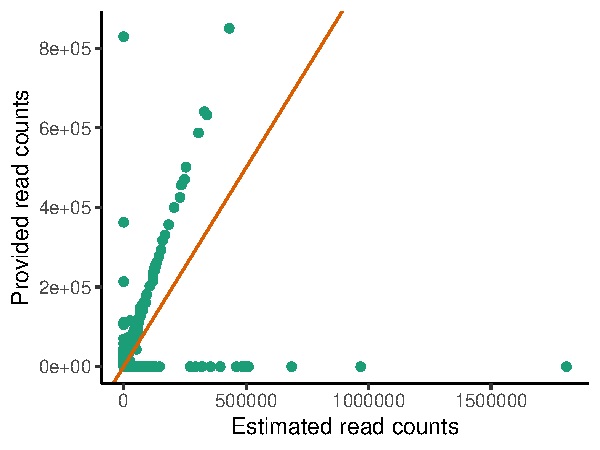
\includegraphics[width=\maxwidth]{figure/count-comparison-1} }\newline
\subfloat[Log-log plot after removing 0 values.\label{fig:count-comparison2}]{\includegraphics[width=\maxwidth]{figure/count-comparison-2} }

}

\caption[Comparison between the estimated counts and the provided values]{Comparison between the estimated counts and the provided values.}\label{fig:count-comparison}
\end{figure}


\end{knitrout}

\section{}

\subsection{Read coverage and library complexity}
To analyse the read coverage, we created the histogram in figure~\ref{fig:read-coverage}. We can see that the count values range from roughly 40 million to 180 million.
We can also see that most samples have more than 60 million reads, although a very small number has only around 40 million.
This might mean that in these samples lowly expressed genes are below the detection threshold. We can also see that there are a lot more genes with read counts in the 60 to 100 million range than in the rest of the domain, which indicates that we will probably need some kind of normalisation of the data.

\begin{knitrout}
\definecolor{shadecolor}{rgb}{0.969, 0.969, 0.969}\color{fgcolor}\begin{figure}[ht]

{\centering \includegraphics[width=\maxwidth]{figure/read-coverage-1} 

}

\caption[Read counts histogram]{Read counts histogram.}\label{fig:read-coverage}
\end{figure}


\end{knitrout}

Library complexity refers to the number of unique DNA fragments present in a given library. To compute library complexity, we used a sampling-based approach. For tissue sample, we sampled the genes with probability proportional to the read count of each gene for that patient. In figure~\ref{fig:library-complexity} we plot the library complexities for all samples.
Analysing the figure we can see that, in general, in samples from normal tissues we hit more genes with fewer samples, which means that the genes are more uniformly represented. On the other hand, in deseased tissues, we get a lower percentage of all the detected genes with the same number of samples, showing that the read counts for the genes in deseased tissues is farther from a uniform distribution: there are a few genes with a much higher read count than the others.


\begin{knitrout}
\definecolor{shadecolor}{rgb}{0.969, 0.969, 0.969}\color{fgcolor}\begin{figure}[ht]

{\centering \includegraphics[width=\maxwidth]{figure/library-complexity-1} 

}

\caption[Library complexity plot]{Library complexity plot.}\label{fig:library-complexity}
\end{figure}


\end{knitrout}

\subsection{Normalisation of the data}
To normalise the data, we used the Trimmed Mean of M (TMM) method. In order to evaluate our normalisation, we produced a series of plots which help us visualise how the data changed after the normalisation.

First, we plotted the histogram of the normalised read counts. When compared with the histogram resulting of the raw read counts (in figure~\ref{fig:read-coverage}), we can se that .....
% TODO MACF plot histogram of the normalised read counts (hopefully it is flatter)
\todo{MACF: plot histogram of the normalised read counts (hopefully it is flatter)}


We produced a plot where the distance between samples corresponds to the leading Biological Coefficient of Variation (BCV), using the function \texttt{plotMDS}. The result can be seen in figure~\ref{fig:mds}. There is a clear separation between the samples of normal tissues and the samples taken from tumours. It also appears that there are two distinct groups of samples from tumours.

Finally, we wanted to ensure that after normalisation there was no difference between the highly expressed and lowly expressed genes. To so so, we coloured the marks according to their read count.........

% TODO MACF different colours for 2 groups of genes with varying number read counts: produce histogram with the columns on the right in one color and the columns on the left another column (separate by mode/median=?). Then plotMDS using the same colours for the respetive marks.
\todo{MACF: different colours for 2 groups of genes with varying number read counts: produce histogram with the columns on the right in one color and the columns on the left another column (separate by mode/median=?). Then plotMDS using the same colours for the respetive marks.}

\begin{knitrout}
\definecolor{shadecolor}{rgb}{0.969, 0.969, 0.969}\color{fgcolor}\begin{figure}[ht]

{\centering \includegraphics[width=\maxwidth]{figure/mds-1} 

}

\caption[Multidimensional Scaling plot of the data after normalizing]{Multidimensional Scaling plot of the data after normalizing.}\label{fig:mds}
\end{figure}


\end{knitrout}

\subsection{Phenotypic traits and genes that dominate variance} % 2c)
  
% TODO MACF try to identify what separates the 2 groups of tumours in the MDS plot.
\todo{MACF: try to identify what separates the 2 groups of tumours in the MDS plot.}
\subsection{} % 2d)

\section{} % Group 3

\subsection{Can genes recapitulate related immunohistochemistry tests} %3a)

We want to show how the gene expression for some genes relates to the binary classification for the related immunohistochemistry-based tests in the patient data. To do so, we produce 3 plots, showed in figure~\ref{fig:3a}.

First, in figure~\ref{fig:3a1} we have a scatter tissue sample the read count of ESR1 on the x-axis and the read count of ERS2 on the y-axis. Each mark is colored according to the presence of estrogen receptors in the respective tissue sample. We can see by this graph that the expression of ESR1 is highly related to the presence of estrogen receptors: the tissue samples with estrogen receptors tend to have higher read counts of ESR1. On the other hand, ESR2 appears to have little influence on the presence of estrogen receptors. We conclude ERS1's expression is very good at recapitulating the presence of estrogen receptors in a tissue sample, but the same is not true of ESR2.

Secondly, in figure~\ref{fig:3a2} we want to evaluate how PGR relates to the presence of progesterone receptors in tissue samples. Since we only have one gene to evaluate, we adopt a different approach: we used a histogram to plot the number of tissue samples we have (in the y-axis) against the read count of PGR. As we can see, the trend is for the tissue samples that test positive for the presence of progesterone receptors to have a higher read count of PGR, and for the the negative samples to have lower values.  We conclude PGR's expression is very good at recapitulating the presence of progesterone receptors in a tissue sample.

Finally, in figure~\ref{fig:3a3} we use a similar histogram to show the relation between the presence of HER2 protein in the tissue sample to the read count of ERBB2 gene.

\begin{knitrout}
\definecolor{shadecolor}{rgb}{0.969, 0.969, 0.969}\color{fgcolor}\begin{figure}[ht]

{\centering \subfloat[Relation between ESR1/ESR2 expression and the presence of estrogen receptors\label{fig:3a1}]{\includegraphics[width=\maxwidth]{figure/3a-1} }\newline
\subfloat[Relation between PGR expression and the presence of progesterone receptors\label{fig:3a2}]{\includegraphics[width=\maxwidth]{figure/3a-2} }\newline
\subfloat[Relation between ERBB2 expression and the presence of HER2 protein\label{fig:3a3}]{\includegraphics[width=\maxwidth]{figure/3a-3} }

}

\caption[Relation between the cognate genes and the immunohistochemistry-based tests]{Relation between the cognate genes and the immunohistochemistry-based tests.}\label{fig:3a}
\end{figure}


\end{knitrout}

\todo{MACF: try to add ROC curves to these plots, or alternatively create another plot with ROC curves.}

\subsection{Survival analysis} %3b)
Just do the survival analysis according to the PAM50 groups.

\begin{knitrout}
\definecolor{shadecolor}{rgb}{0.969, 0.969, 0.969}\color{fgcolor}\begin{figure}[ht]

{\centering \includegraphics[width=\maxwidth]{figure/survival-1} 

}

\caption[Hello]{Hello}\label{fig:survival}
\end{figure}


\end{knitrout}

\subsection{Gene signature that best classifies molecular subtypes} %3c)

\begin{knitrout}
\definecolor{shadecolor}{rgb}{0.969, 0.969, 0.969}\color{fgcolor}\begin{figure}[ht]

{\centering \includegraphics[width=\maxwidth]{figure/unnamed-chunk-3-1} 

}

\caption[Hello]{Hello}\label{fig:unnamed-chunk-31}
\end{figure}

\begin{figure}[ht]

{\centering \includegraphics[width=\maxwidth]{figure/unnamed-chunk-3-2} 

}

\caption[Hello]{Hello}\label{fig:unnamed-chunk-32}
\end{figure}


\begin{tabular}{lrrrrrr}
\toprule
  & logFC & AveExpr & t & P.Value & adj.P.Val & B\\
\midrule
FOXC1 & -3.982 & 3.321 & -15.80 & 0 & 0 & 101.94\\
SFRS13B & -1.941 & 0.854 & -15.29 & 0 & 0 & 95.74\\
MLPH & 4.168 & 7.127 & 15.03 & 0 & 0 & 92.64\\
SIDT1 & 3.183 & 4.731 & 14.59 & 0 & 0 & 87.45\\
FOXA1 & 5.231 & 7.212 & 14.48 & 0 & 0 & 86.20\\
\addlinespace
PRR15 & 4.545 & 3.818 & 14.46 & 0 & 0 & 85.99\\
AR & 4.472 & 4.215 & 14.43 & 0 & 0 & 85.65\\
ERBB2 & 3.179 & 8.391 & 14.18 & 0 & 0 & 82.80\\
PGAP3 & 2.555 & 5.432 & 14.10 & 0 & 0 & 81.89\\
ABCC11 & 6.595 & 3.436 & 14.06 & 0 & 0 & 81.46\\
\bottomrule
\end{tabular}


\end{knitrout}

\subsection{Classifying molecular subtype} %3d)
\end{document}
